\documentclass[../ECE459FinalProjectReport.tex]{subfiles}

\begin{document}
\chapter{Results}
\section{Experiment Settings}
%todo: 写实验所使用的信号及表达式、载波参数、调制系数等等
\subsection{The Message Signal}
Considering the wide application of AM/FM technologies in radio communication where the data to transmit is mainly human voice, this project applies a TTS-generated monaural male voice recording which samples at \SI{48}{kHz} and lasts around \SI{3.5}{s}.

The bandwidth of the TTS-generated recording can be determined by its spectrum illustrated in Figure \ref{fig:audio-original} using Python. Note that the recording is generated using the male's voice, which typically ranges from \SI{80}{Hz} to \SI{200}{\Hz}. It is observed that the majority of power is concentrated within \SI{5}{kHz}, which will be regarded as the bandwidth of the message signal. To ensure a more precise bandwidth, an LPF is added to remove unnecessary frequency components beyond \SI{5}{kHz}.
\begin{figure}[hb]
    \centering
    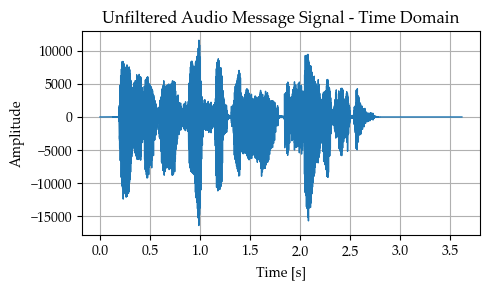
\includegraphics[width=0.49\linewidth]{plots/unfiltered_audio_time.png}
    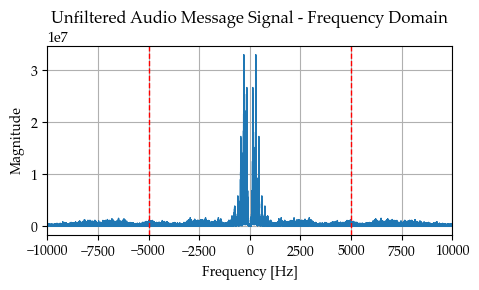
\includegraphics[width=0.49\linewidth]{plots/unfiltered_audio_freq.png}
    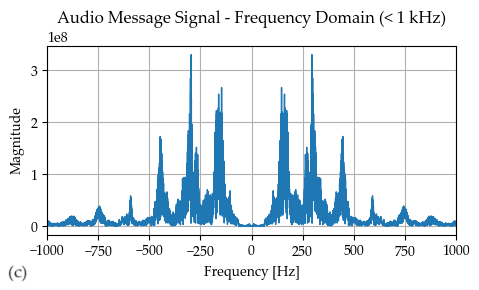
\includegraphics[width=0.49\linewidth]{plots/audio_spectrum_1khz.png}
    \caption{The waveforms of the unfiltered audio recording. (a) The signal in time domain. (b) The spectrum of the signal. The majority of the response is concentrated within \SI{1}{kHz}, but the team chooses \SI{5}{kHz} for balancing better audio quality and bandwidth saving. (c) The spectrum of the signal within \SI{1}{kHz}. The major frequency components are among \qtyrange{125}{500}{Hz}.}
    \label{fig:audio-original}
\end{figure}

\subsection{Simulation Parameters}
\subsubsection{AM Simulation}
The parameters for AM simulation are listed as follows:
\begin{itemize}
    \item Message Bandwidth $f_m = \SI{5}{kHz}$.
    \item Message Amplitude $A_m=11604$.
    \item Sampling Frequency $f_s = \SI{48}{kHz}$.
    \item Modulation Index $\mu = 0.3$.
    \item Carrier Wave Frequency $f_c = \SI{12}{kHz}$.
    \item Carrier Wave Amplitude $A_c = 1$.
    \item Variance of AWGN $\sigma^2 = \num{1e-5}$.
\end{itemize}
Using the parameters above, the following parameters can be calculated:
\begin{itemize}
    \item Modulation Sensitivity $k_a = \num{1.83e-5}$.
\end{itemize}

\subsubsection{FM Simulation}
The parameters for FM simulation are listed as follows:
\begin{itemize}
    \item Message Bandwidth $f_m = \SI{5}{kHz}$.
    \item Message Amplitude $A_m=11604$.
    \item Sampling Frequency $f_s = \SI{480}{kHz}$.
    \item Modulation Index $\beta=0.3$.
    \item Carrier Wave Frequency $f_c = \SI{180}{kHz}$.
    \item Carrier Wave Amplitude $A_c = 1$.
    \item Variance of AWGN $\sigma^2 = \num{1e-7}$ ($\sigma^2=\num{1e-5}$ is also tested).
\end{itemize}
Using the parameters above, the following parameters can be determined:
\begin{itemize}
    \item Maximum Frequency Deviation $\Delta f=\beta f_m = \SI{1.5}{kHz}$.
    \item Transmission Bandwidth $B_T = 2\left( \Delta f + f_m\right) = \SI{13}{kHz}$.
    \item Modulation Sensitivity $k_f = 0.129$.
\end{itemize}

\section{AM Simulation}
To maximally eliminate the distortion at the beginning and end of the time domain signal brought by the filters, the message signal is padded with zeros at both the beginning and the end. The signal is shown in Figure \ref{fig:am-long-message}.

The zero-padded message signal is then modulated with the carrier wave, and the modulated signal is shown in Figure \ref{fig:am-modulated}. Note that the spectrum of the modulated signal has frequency components around the carrier frequency \SI{12}{kHz}.

The noise is then added to the signal and produces a noisy FM signal. The signal is illustrated \ref{fig:noisy-am}.

At the receiver side, a BPF is applied to the signal to suppress noise. The spectrum of the filtered signal is shown in Figure \ref{fig:noisy-am-filtered}. Then the envelope detector is applied to the signal, which produces the demodulated signal shown in Figure \ref{fig:am-demodulated}.

The SNRs are calculated to be:
\begin{itemize}
    \item Pre-Detection SNR: \SI{46.99}{dB}.
    \item Post-Detection SNR: \SI{119.96}{dB}.
\end{itemize}

The team also tried different pre- and post-detection SNRs. The visual diagram of the relation between pre- and post-detection SNRs is shown in Figure \ref{fig:am-snr-relation}. They are almost linear with each other, which matches the theoretical computation in \cite[Sec. 9.7]{haykinIntroductionAnalogDigital2007}

\begin{figure}[b]
    \centering
    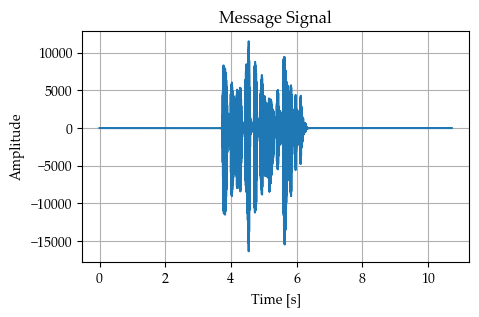
\includegraphics[width=0.49\linewidth]{plots/am/message_time.png}
    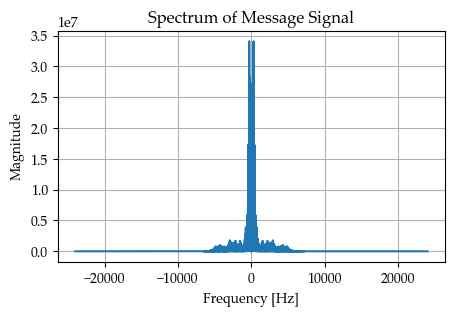
\includegraphics[width=0.49\linewidth]{plots/am/message_spectrum.png}
    \caption{The zero-padded message signal. It is triple the length of the original message signal.}
    \label{fig:am-long-message}
\end{figure}
\begin{figure}[b]
    \centering
    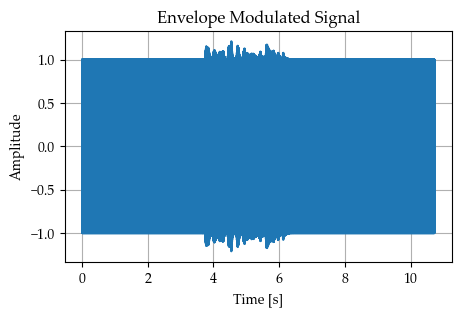
\includegraphics[width=0.49\linewidth]{plots/am/modulated_time.png}
    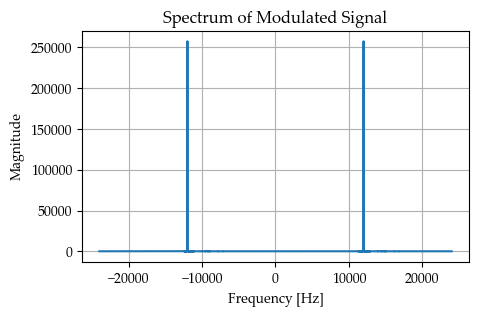
\includegraphics[width=0.49\linewidth]{plots/am/modulated_spectrum.png}
    \caption{The envelope-modulated signal.}
    \label{fig:am-modulated}
\end{figure}
\begin{figure}[b]
    \centering
    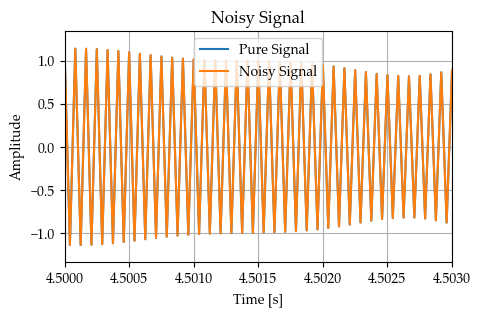
\includegraphics[width=0.49\linewidth]{plots/am/noisy_time.png}
    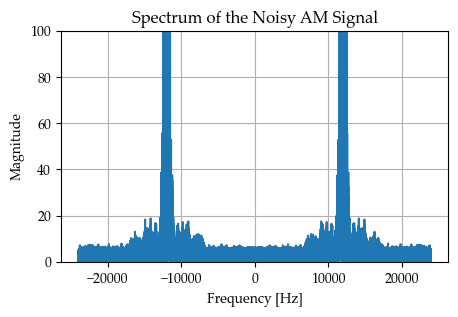
\includegraphics[width=0.49\linewidth]{plots/am/noisy_spectrum.png}
    \caption{The noisy AM signal. Note that the plotting magnitude range of the spectrum is limited in order to show the noise clearly.}
    \label{fig:noisy-am}
\end{figure}
\begin{figure}[b]
    \centering
    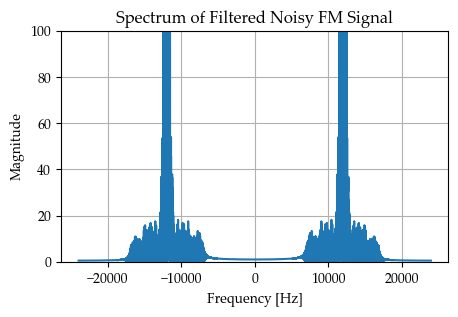
\includegraphics[width=0.6\linewidth]{plots/am/noisy_spectrum_filtered.png}
    \caption{The filtered noisy AM signal.}
    \label{fig:noisy-am-filtered}
\end{figure}
\begin{figure}[b]
    \centering
    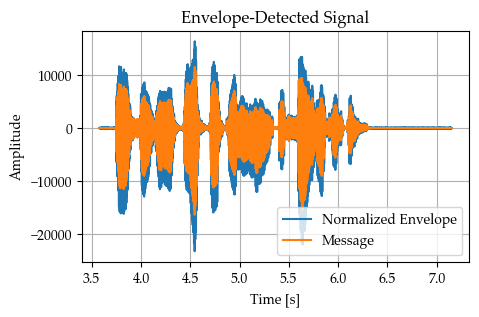
\includegraphics[width=0.49\linewidth]{plots/am/detected_time.png}
    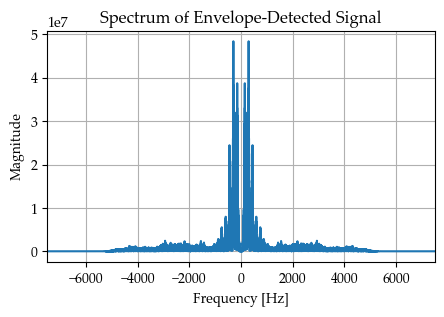
\includegraphics[width=0.49\linewidth]{plots/am/detected_spectrum.png}
    \caption{The demodulated signal of AM system.}
    \label{fig:am-demodulated}
\end{figure}
\begin{figure}[b]
    \centering
    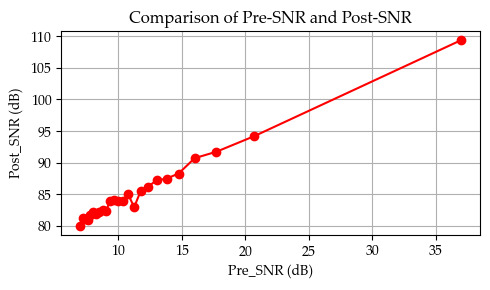
\includegraphics[width=0.6\linewidth]{plots/am/am_snr_relation.png}
    \caption{The relationship between AM pre- and post-detection SNRs.}
    \label{fig:am-snr-relation}
\end{figure}

\section{FM Simulation}
The same audio file is applied as the input to the system, whose time and frequency domain waveforms are shown in Figure \ref{fig:audio-spectrum}. In order to reach the target sampling frequency \SI{48}{kHz}, the team first did an upsample by a factor of 10 to the audio by \verb|scipy.signal.resample()|. This allows the team to have better flexibility in designing filters. The upsampling expands the frequency spectrum by the properties of the Fast Fourier Transform (FFT) Algorithm. The spectrum of resampled and filtered signal is shown in Figure \ref{fig:audio-spectrum}. Note that compared to Figure \ref{fig:audio-original}(b), the magnitude for each frequency component is multiplied by a factor of 10.
\begin{figure}[tb]
    \centering
    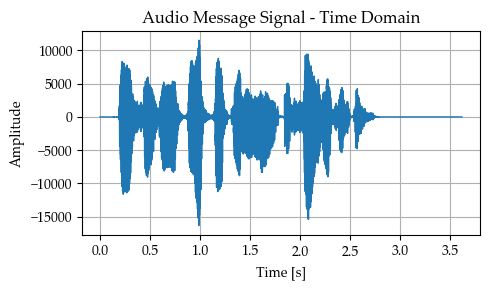
\includegraphics[width=0.49\linewidth]{plots/audio_time.png}
    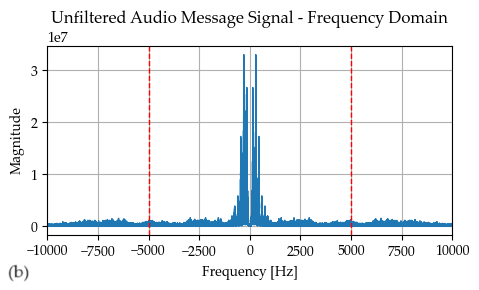
\includegraphics[width=0.49\linewidth]{plots/audio_spectrum.png}
    \caption{The waveforms of the resampled \SI{5}{kHz} low-pass filtered audio recording. (a) The signal in time domain. (b) The spectrum of the signal.}
    \label{fig:audio-spectrum}
\end{figure}

The integrator takes an integral to the message signal, and the controllable oscillator produces the frequency-modulated signal. The waveform and the spectrum of the signal are shown in Figure \ref{fig:fm-signal} and \ref{fig:fm-spectrum-tx-bw}. The two main lobes present around the carrier frequency $f_c = \SI{180}{kHz}$.

The noise is the same as the AM simulation, and the noisy frequency-modulated signal is shown in Figure \ref{fig:noisy-fm}. After receiving the signal, the signal is band-pass filtered and the signal is shown in Figure \ref{fig:fm-bpf}. The pass-band of the filter is designed to be from $f_c - B_T$ to $f_c + B_T$, where $B_T$ is the transmission bandwidth. The filtered signal is then taken differentiation and envelope detection (using ideal envelope detector realised by Hilbert transformation), and the results are shown in Figure \ref{fig:fm-diff} and Figure \ref{fig:envelope} respectively.

After steps above, we use low pass filter at first, and then minus the DC value bias directly to get the fully recovered signal (see Figure \ref{fig:fm-result}).

The final result we get for the SNR is like this:
\begin{itemize}
    \item Pre-Detection SNR: \SI{66.99}{dB}.
    \item Post-Detection SNR: \SI{258.64}{dB}.
\end{itemize}
As we can see, the post-SNR is obviously much higher than the post one. Because while the lowpass filter does not damage the message signal, the power for the noise is significantly decreased.

In order to compare the anti-noise performance with AM, the team tested the noise variance $\sigma^2 = \num{1e-5}$. The pre-detection SNR in this case is \SI{46.99}{dB}, and the post-detection SNR is \SI{239.792}{dB}. The post-detection SNR is much higher than AM, which indicates FM has better anti-noise performance.

The relationship between pre- and post-detection SNRs is tested and plotted in Figure \ref{fig:fm-snr-relation}.

\begin{figure}[tb]
    \centering
    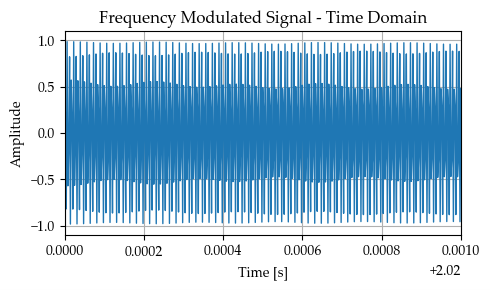
\includegraphics[width=0.49\linewidth]{plots/fm/fm_time_smallInterval.png}
    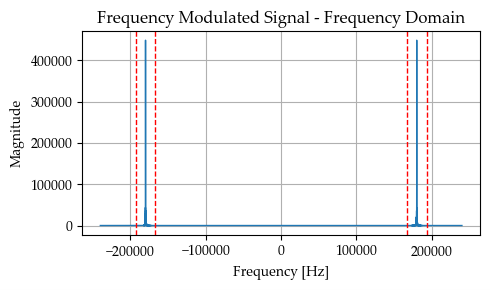
\includegraphics[width=0.49\linewidth]{plots/fm/fm_freq.png}
    \caption{The waveform and spectrum of the frequency-modulated signal.}
    \label{fig:fm-signal}
\end{figure}
\begin{figure}[tb]
    \centering
    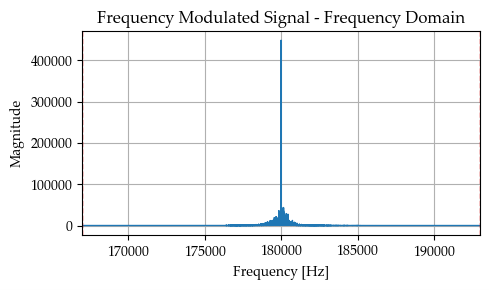
\includegraphics[width=0.49\linewidth]{plots/fm/fm_freq_bt.png}
    \caption{The spectrum of the frequency-modulated signal within the transmission bandwidth.}
    \label{fig:fm-spectrum-tx-bw}
\end{figure}
\begin{figure}[tb]
    \centering
    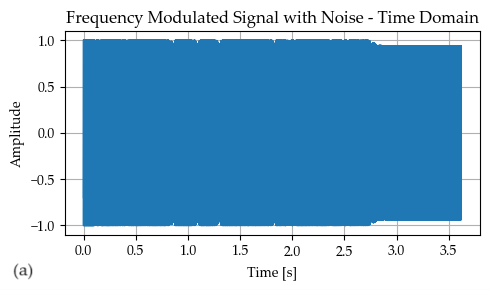
\includegraphics[width=0.49\linewidth]{plots/fm/noisy_fm_time.png}
    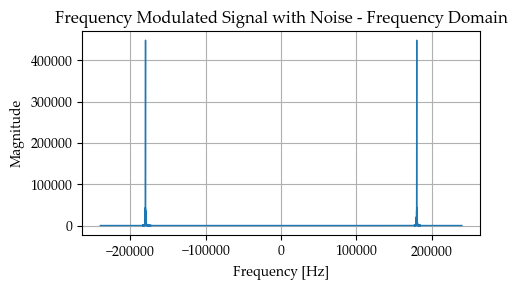
\includegraphics[width=0.49\linewidth]{plots/fm/noisy_fm_freq.png}
    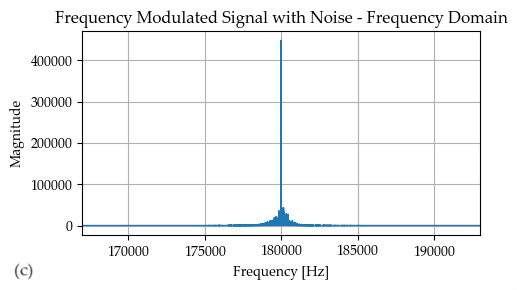
\includegraphics[width=0.49\linewidth]{plots/fm/noisy_fm_freq_bw.png}
    \caption{The waveforms of the noisy frequency-modulated signal. (a) The time-domain signal. (b) The frequency-domain signal. (c) The frequency-domain signal within the transmission bandwidth. Note that the response is non-zero beyond the transmission bandwidth.}
    \label{fig:noisy-fm}
\end{figure}
\begin{figure}[tb]
    \centering
    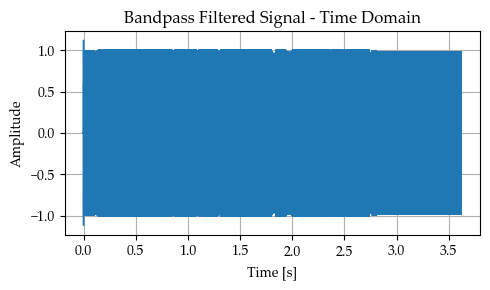
\includegraphics[width=0.49\linewidth]{plots/fm/bpf_signal_time.png}
    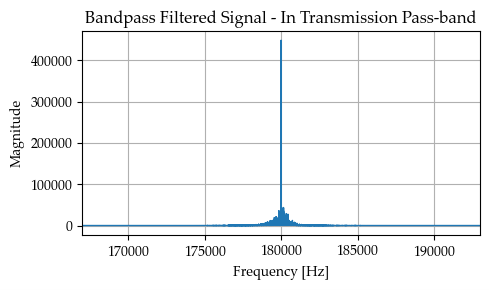
\includegraphics[width=0.49\linewidth]{plots/fm/bpf_signal_freq_bw.png}
    \caption{The band-pass filtered frequency-modulated signal. Note that some distortion happens at the beginning of the signal, which is brought about by filtering a non-periodic signal using a digital filter.}
    \label{fig:fm-bpf}
\end{figure}
\begin{figure}[tb]
    \centering
    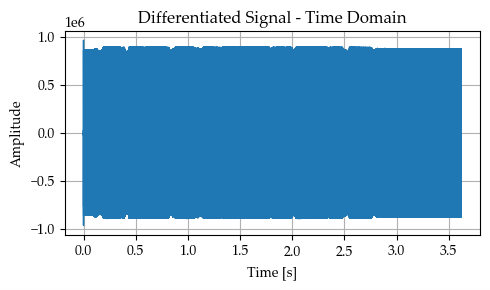
\includegraphics[width=0.49\linewidth]{plots/fm/diff_signal_time.png}
    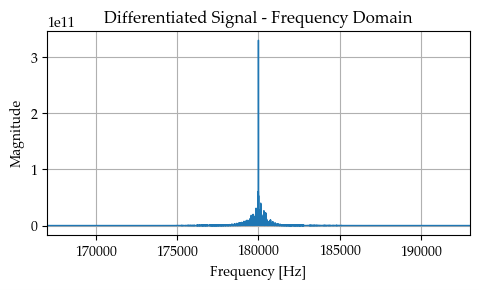
\includegraphics[width=0.49\linewidth]{plots/fm/diff_signal_freq_bw.png}
    \caption{The differentiated signal.}
    \label{fig:fm-diff}
\end{figure}
\begin{figure}[tb]
    \centering
    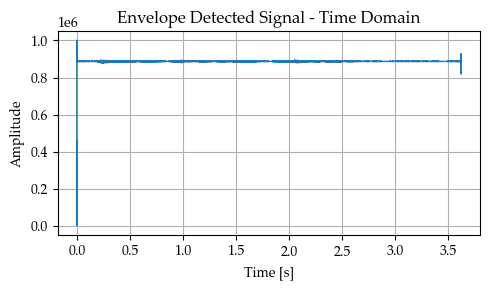
\includegraphics[width=0.49\linewidth]{plots/fm/envelope_signal_time.png}
    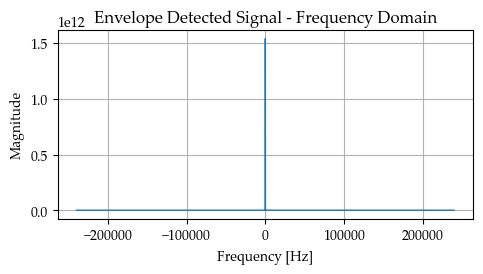
\includegraphics[width=0.49\linewidth]{plots/fm/envelope_signal_freq.png}
    \caption{The envelope detected differentiated signal. Note that the signal has a non-zero DC offset compared to the message signal.}
    \label{fig:fm-envelope}
\end{figure}
\begin{figure}[tb]
    \centering
    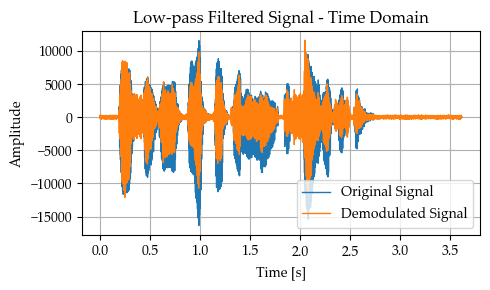
\includegraphics[width=0.49\linewidth]{plots/fm/lpf_signal_time.png}
    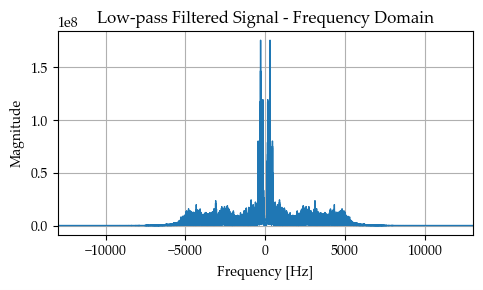
\includegraphics[width=0.49\linewidth]{plots/fm/lpf_signal_freq_smallFreq.png}
    \caption{The low-pass filtered and DC-blocked signal with maximum amplitude matched with the message signal.}
    \label{fig:fm-result}
\end{figure}

\begin{figure}[tb]
    \centering
    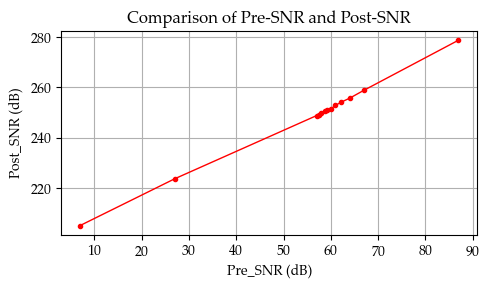
\includegraphics[width=0.49\linewidth]{plots/fm/snr1.png}
    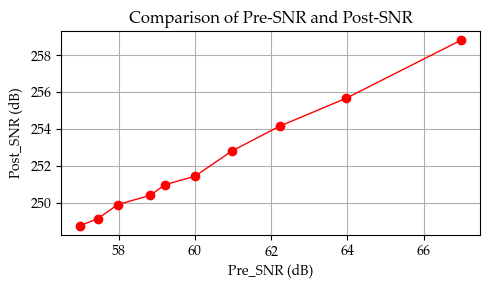
\includegraphics[width=0.49\linewidth]{plots/fm/snr2.png}
    \caption{The plot of FM pre-detection SNR vs. post-detection SNR.}
    \label{fig:fm-snr-relation}
\end{figure}
\end{document}